% Chapter Template

\chapter{Conclusions and Future Work} % Main chapter title %% EXTRACT RESULTS SECTION FROM HERE TO NEW CHAPTER

\label{Chapter6} % Change X to a consecutive number; for referencing this chapter elsewhere, use \ref{ChapterX}

%----------------------------------------------------------------------------------------
%	SECTION 1   % TARGET 1500 WORDS IN THIS CHAPTER
%----------------------------------------------------------------------------------------

\section{Overview}
This chapter provides concluding remarks on the deliverables of the project and provides a discussion on aspects where the project might benefit moving forward.

%----------------------------------------------------------------------------------------
%	SECTION 2
%----------------------------------------------------------------------------------------

\section{MEGAphone Chassis/Case First Revision}
The MEGAphone accessible interface project was fully realised on the 8th of November, 2020.
In this chapter, the development of the project and how various aspects benefit the usability and sovereignty of the MEGAphone project, will be summarised. % maybe add to overview
Additionally, a discussion on the potential future work of the project will establish how to best approach a succeeding revision of the chassis and the MEGAphone PCB followed by some concluding remarks.

% %-----------------------------------
% %	SUBSECTION 1
% %-----------------------------------
\subsection{Research Questions}

This thesis has answered the following research questions in the preceding chapters:
\begin{enumerate}
    \item What is the relationship between Digital Sovereignty and Universal Design?
        \begin{enumerate}
        \item[-] Chapter one introduced these concepts and their characteristics.
        \item[-] Chapter two set out to establish what each of these concepts meant along with their importance in this project.
        \item[-] Chapter four took those concepts and applied them to a real tangible design, drawing commonality between these concepts along the way.
        \end{enumerate} 
    \item Why is Universal Design important in the design of products today?
        \begin{enumerate}
        \item[-] Chapter two established why UD is important, as the concept attempts to normalise accessible design practices so that people with a disability or of old age can be better included in the products of today.
        \item[-] Chapter four applied that concept, highlighting the importance of such features and how not only those with a disability, but also abled bodied people can benefit. 
        \end{enumerate}
    \item Why is Digital Sovereignty important in the design of electronic products today?
        \begin{enumerate}
        \item[-] Chapter two covers the MEGAphone mobile device and how users can benefit from an open and secure platform.
        \item[-] Chapter three explained how considering open-source software in the development of the project can make it easier for users to modify aspects of the product after the fact.
        \item[-] Chapter four presented examples of DS in practice, such as the solar cell feature, which provides users with an alternative way to charge their device, making them no longer solely dependent on a working energy infrastructure.
        \end{enumerate} 
    \item How can the seven design principles be used in the design of the MEGAphone case to support those with disabilities?
        \begin{enumerate}
        \item[-] Chapter one introduces the seven design principles as a tool to measure the accessibility of a product.
        \item[-] Chapter two goes into detail on these principles and briefly explains the characteristics of each design principle.
        \item[-] Chapter four provides evidence of the seven design principles in practice, highlighting how they apply to each design feature.
        \end{enumerate} 
    \item How can the 'Right to Repair' philosophy be used in support of the universally designed MEGAphone case?
        \begin{enumerate}
        \item[-] Chapter two discussed how planned obsolescence works in favour of the manufacturer and against the user and the freedoms that the user gives up as a result.
        \item[-] Chapter four provides evidence as to how this philosophy can support the project, such as making the internal components easy to access to those who desire access, while not sacrificing safety for those who don't, as per the UD concept.
        \end{enumerate} 
    \item What are the effects of COVID-19 on Digital Sovereignty, Universal Design and the MEGAphone project?
        \begin{enumerate}
        \item[-] Chapter two looks at the effects of COVID-19 related to capability maintenance and what this potentially means for people with a disability.
        \item[-] Chapter four explains that this pandemic disrupted the iterative design process as focus groups consisting of people with disabilities for design feedback was abandoned due to the health risks of the virus.
        \end{enumerate} 
\end{enumerate}

% %-----------------------------------
% %	SUBSECTION 2
% %-----------------------------------
\subsection{Contributions to the Field}

The author's key contributions to the field, recounted in detail, are:
\begin{enumerate}
    \item An examination of the relationship between Digital Sovereignty and Universal Design.
        \begin{enumerate}
        \item[-] As recounted in the previous subsection, this thesis provides a comprehensive examination of the UD and DS concepts and the relationship that they share.
        \end{enumerate} 
    \item Analysis of the existing MEGAphone PCB design from the perspective of UD.
        \begin{enumerate}
        \item[-] This project delivers three new PCB designs, to interface with the existing PCB, in order to better adapt it to the principles of UD.
        \end{enumerate} 
    \item The creation through iteration of a UD housing for the MEGAphone PCB.
        \begin{enumerate}
        \item[-] Chapter four provides a comprehensive review of the UD housing for the MEGAphone project, including evidence of an iterative design process.
        \item[-] Chapter five further supports this by providing the CAD work for a future 3D-print of the project.
        \end{enumerate} 
    \item The improvement of the MEGAphone device layout to improve its UD properties.
        \begin{enumerate}
        \item[-] Evidence of this during the project is presented in the form of smaller external PCBs that serve to interface with the main PCB for the sake of delivering an accessible prototype, thereby avoiding a costly and time-consuming redesign of the MEGAphone.
        \item[-] The implementation of the 'EZ access keys' provides the MEGAphone device with a useful alternative method of use which supports UD principles.
        \item[-] Accompanying the 'EZ access keys' is the adaptation of large rocker switches which make controlling power to various modules of the MEGAphone far easier than previously possible.
        \item[-] Hardware-implemented 'software' features transparent to the MEGA65 OS provide users with an alternative method of interacting with the keyboard, through the use of a Jellybean switch.
        \end{enumerate} 
    \item The design of practical modifications to the MEGAphone PCB design that allows the majority of the UD improvements to be realised, without requiring a complete and costly redesign of the MEGAphone PCB.
        \begin{enumerate}
        \item[-] This links closely with the previous contribution where these practical modifications are realised as supporting PCBs which interface with the main PCB.
        \end{enumerate} 
    \item The proposal of further improvements to the MEGAphone PCB and case designs to further improve their UD properties.
        \begin{enumerate}
        \item[-] Recommendations on how to approach a MEGAphone PCB redesign and case in the future, that better satisfies the UD concept is discussed in section 3.2.
        \item[-] Chapter five provides a critical appraisal of the final 3D-printed housing, where improvements to the design in response to the outcome are proposed and presented.
        \end{enumerate} 
    \item The creation of a MEGAphone device prototype, including UD features and housing, that can be used in future UD studies of the MEGAphone.
        \begin{enumerate}
        \item[-] As first presented in chapter four, the main deliverable of this project is the full realisation of an accessible MEGAphone prototype that can be used in future endeavours.
        \end{enumerate} 
\end{enumerate}

%----------------------------------------------------------------------------------------
%	SECTION 3
%----------------------------------------------------------------------------------------
\section{Future Work}
The following section addresses both the MEGAphone PCBs and the accessible chassis with a discussion on the recommendations of the project moving forward.

%-----------------------------------
%	SUBSECTION 1
%-----------------------------------
\subsection{Original PCB Layout}
% analyse the changes in the final design, what limitations the existing PCB layout has and propose a better layout that satisfies the UD principles, talk about what is ideal and what is the best that can be done with the current layout. 
% Ideal layout includes ports at top of device along with rocker switches replacing current rev2 switches on the main PCB
The layout of the second revision MEGAphone PCB served as the major constraint of this project, as the case design had to be designed around it without any significant redesign due to the complexity of the device. 
Certain reworks to better adapt the design to an accessible interface included removing the existing switches in favour of larger rocker switches hosted on an external PCB (view figure).

\begin{figure} [h]
\begin{centering}
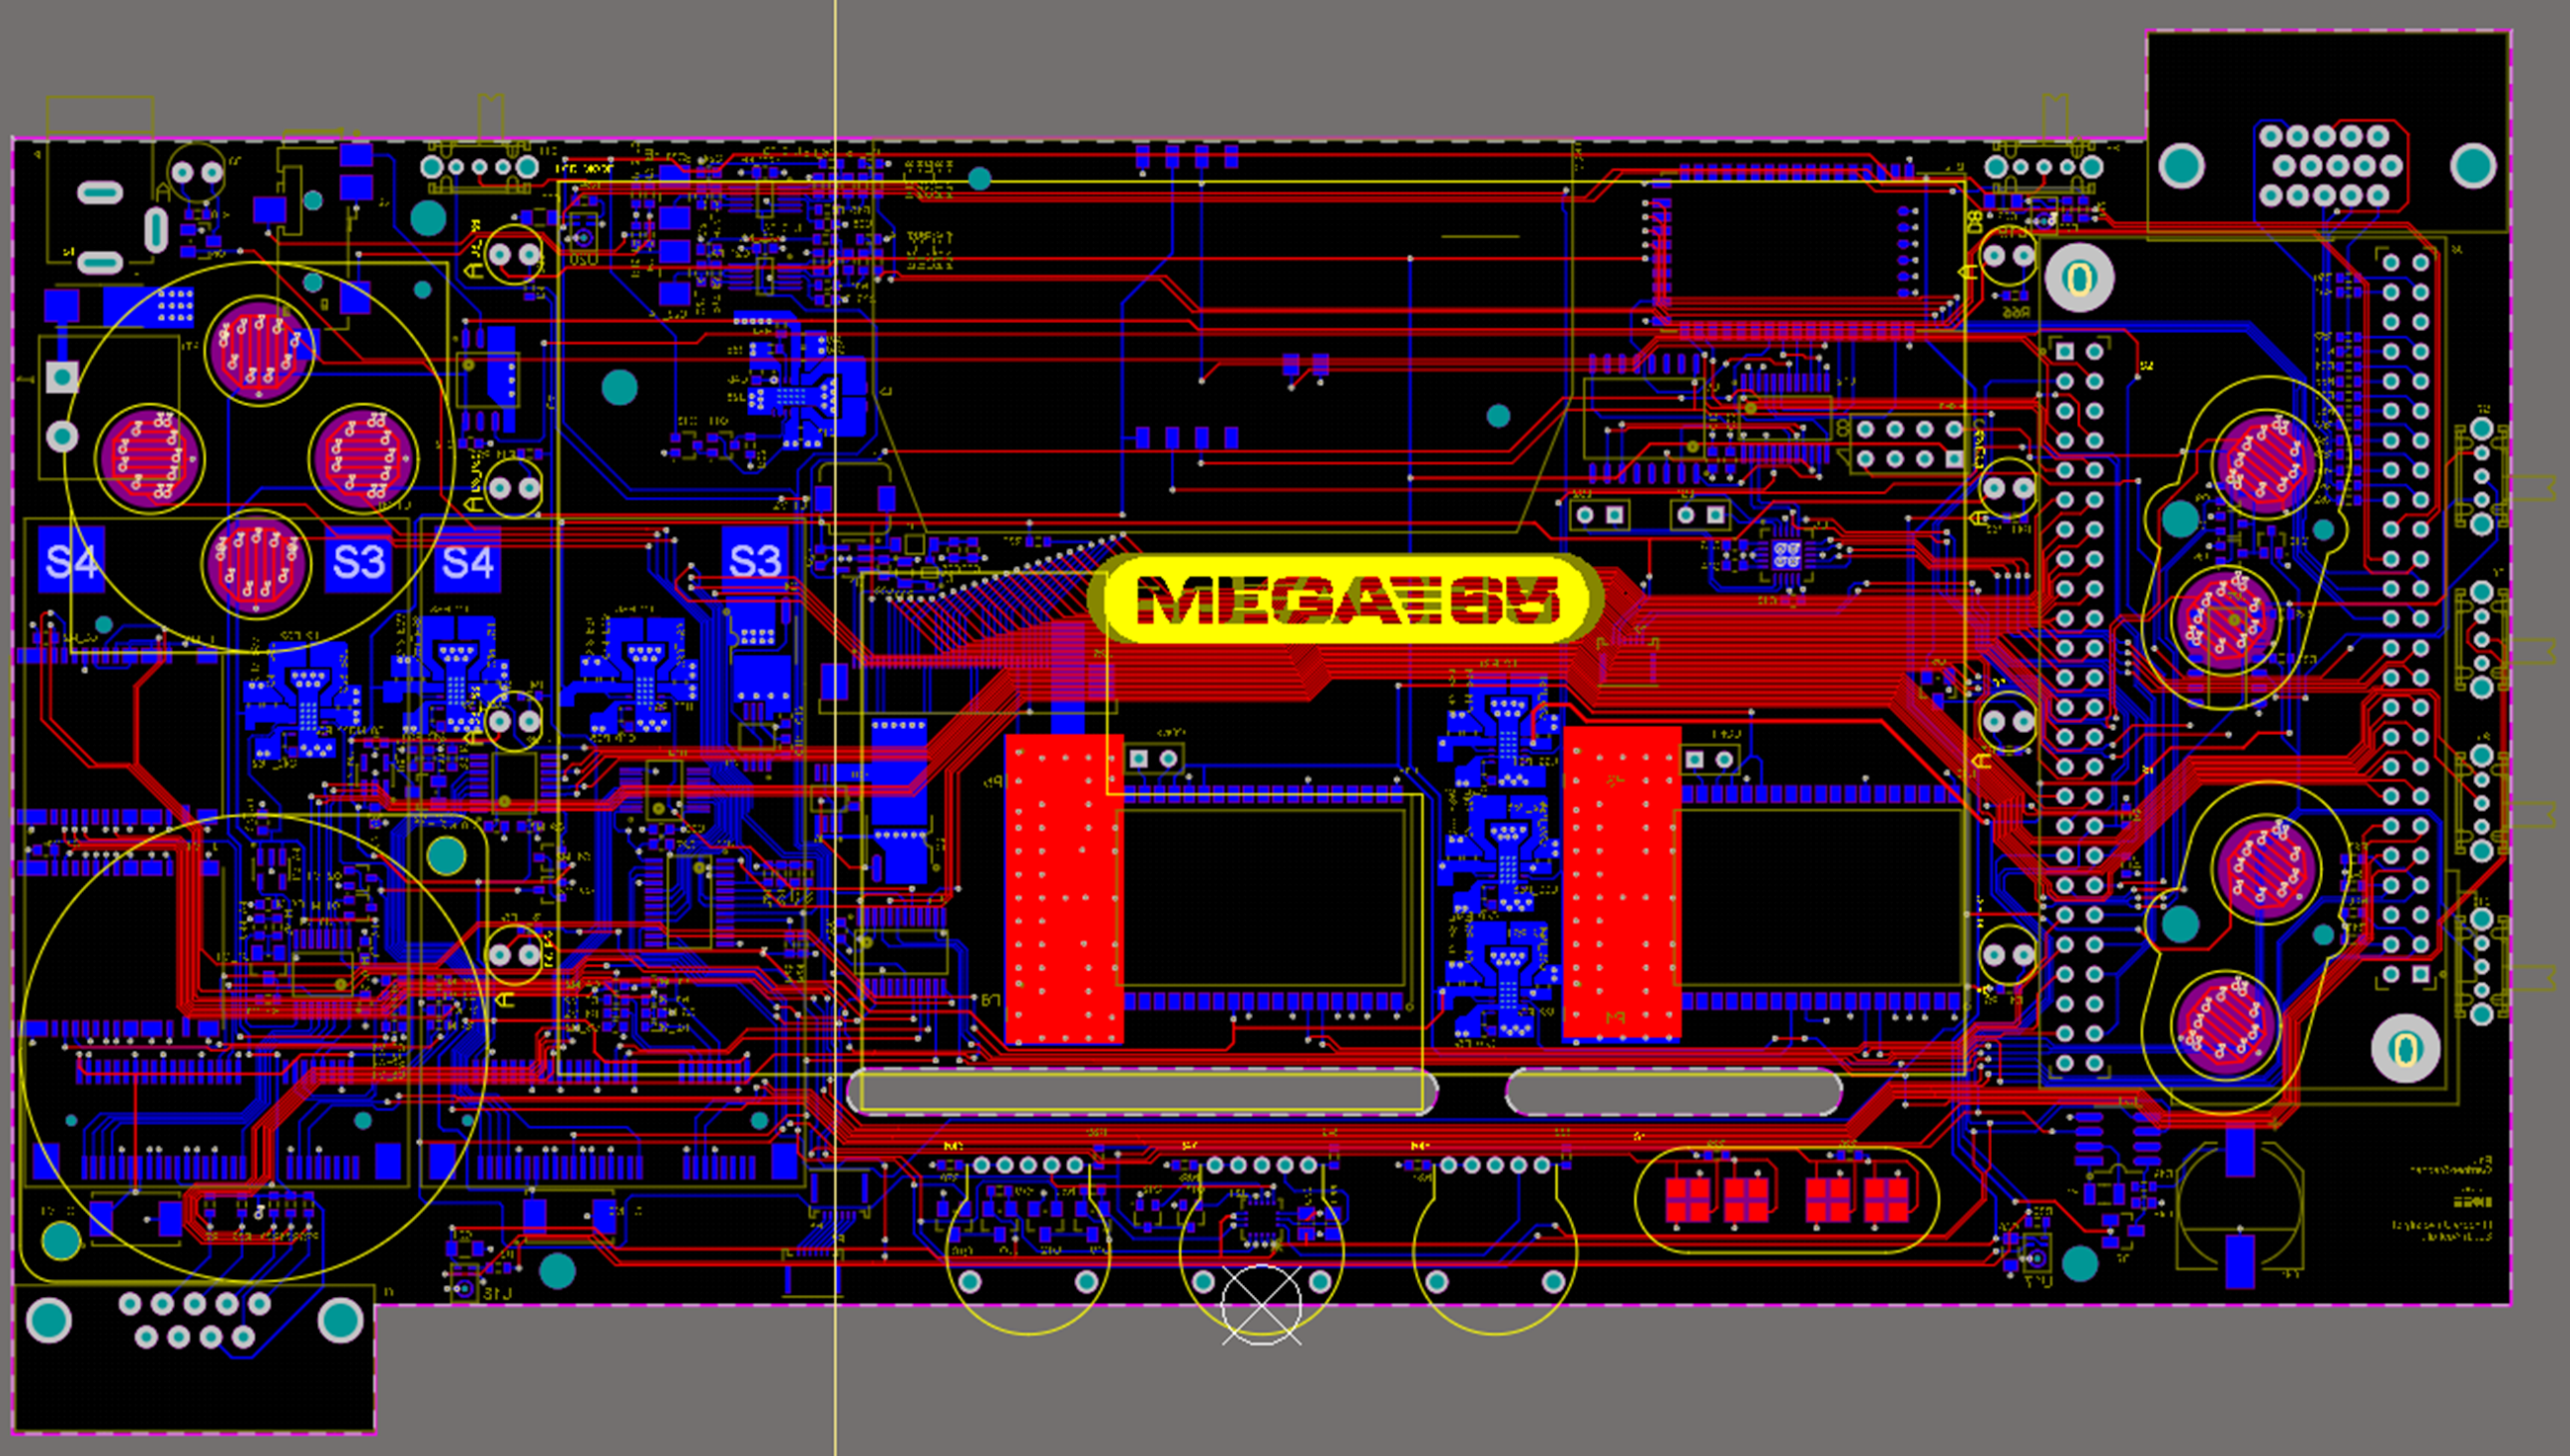
\includegraphics[width=10cm,height=10cm,keepaspectratio]{Figures/pcb_original.png}
\caption{This is the PCB layout as it was during the development of this project.}
\label{fig:ThisFig}
\end{centering}
\end{figure}

%-----------------------------------
%	SUBSECTION 2
%-----------------------------------
\subsection{Proposed PCB Layout}

A possible solution to the existing PCB which does inhabit the Universal Design principles is proposed in figure X. 
The underlying idea with this redesign was to integrate the design all onto one PCB as doing so would reduce the quantity of wires required and given that those in the current solution are soldered to make space, it makes the design overall ‘simpler’.
The reason for the redesign not being undertaken in this project has been discussed previously as impractical due to an issue of cost and time.

\begin{figure} [h]
\begin{centering}
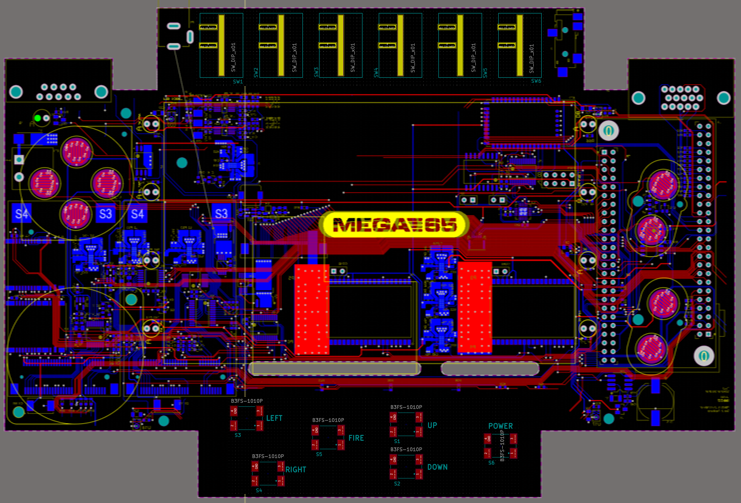
\includegraphics[width=10cm,height=10cm,keepaspectratio]{Figures/pcb_final.png}
\caption{This is the PCB as it is proposed in a future revision of the MEGAphone project.}
\label{fig:ThisFig}
\end{centering}
\end{figure}

In order to make the device more intuitive, placement of the 9-pin DSUB port should be moved to the ‘top’ of the device in the same orientation as the VGA port, so that users know from a glance that this is where all device ports are expected to be.
The accessible button interface also utilises an external PCB which hosts the tactile switches that were opted to form the base of the accessible button function.

Other options were considered, such as silicone rubber pads, as used for the directional button and ‘A’, ‘B’ buttons. 
However, primarily due to the size, larger buttons would be recommended as this would make button presses easier for all users, disregarding the EZ keys in this scenario.
It is acknowledged that larger buttons on the PCB would invalidate the current Gameboy buttons, which is why a complete redesign of those buttons would be recommended to further progress the accessibility of the device as a whole.

It is also recommended that the PCB incorporates multiple 3.5mm jack inputs, separate from the audio function, in its design as this can give users the ability to plug in multiple switches much like the Jellybean presented in this project.
Microsoft's accessible controller \cite{adaptive} is a prime example of the usefulness of this feature and for those who might not be able to interact with the EZ keys or Gameboy buttons but desire their means of interaction with the device, multiple inputs allow for multiple unique functions.
Placement of these inputs should be at the 'top' of the device with all other ports as can be seen in figure X, as this minimises complexity by ensuring that everything is in one place for the user.

%-----------------------------------
%	SUBSECTION 3
%-----------------------------------
\subsection{MEGAphone Housing}

There are a few recommendations regarding the design of the housing for the MEGAphone project.
The space around the power and audio ports of the device could benefit from being better filled in around further working toward a better-sealed device.

The handgrip aspect of the device could also benefit from some refinement as physical use with the device was comfortable, however, it was observed that the grip did not do enough to support user's thumbs.
While the ridges on the 'top' housing fit their purpose in guiding the user's hands to the correct place, they are less important than the ridges at the 'bottom' of the device.
Therefore, more focus on support for the user's thumbs would benefit this project far more.

As previously mentioned, a better interlocking mechanism for the updated solar panel feature would benefit the usability of the device when inserting or removing solar cells.
Additionally, a more refined method of extending out the two device stands would be useful, accompanied by a locking feature for quality of life.
While the current implementation does lock the stand in place to some degree, however, if the device is tilted upside down, this locking mechanism will likely fail.
Ultimately, emphasis should be placed on redesigning the MEGAphone PCB first and foremost.

%----------------------------------------------------------------------------------------
%	SECTION 4
%----------------------------------------------------------------------------------------

\section{Final Summary}
This final concluding chapter recalls the research questions and contributions of the author originally discussed in the first chapter.
Those research questions and contributions were listed in this chapter and provided with short summaries as to how each item was addressed in this thesis.
Future development towards this project was discussed, where the author's opinions on what should be addressed next were provided, with explanations as to why each aspect should be approached in a particular way.
%% FINISH THIS